% This must be in the first 5 lines to tell arXiv to use pdfLaTeX, which is strongly recommended.
\pdfoutput=1
% In particular, the hyperref package requires pdfLaTeX in order to break URLs across lines.

\documentclass[11pt]{article}

% Remove the "review" option to generate the final version.
\usepackage{ACL2023}

% Standard package includes
\usepackage{times}
\usepackage{latexsym}
\usepackage{amsmath}
\usepackage{amssymb}
\usepackage{graphicx}
\usepackage{booktabs}
\usepackage{array}

% For proper rendering and hyphenation of words containing Latin characters (including in bib files)
\usepackage[T1]{fontenc}
% For Vietnamese characters
% \usepackage[T5]{fontenc}
% See https://www.latex-project.org/help/documentation/encguide.pdf for other character sets

% This assumes your files are encoded as UTF8
\usepackage[utf8]{inputenc}

% This is not strictly necessary, and may be commented out.
% However, it will improve the layout of the manuscript,
% and will typically save some space.
\usepackage{microtype}

% This is also not strictly necessary, and may be commented out.
% However, it will improve the aesthetics of text in
% the typewriter font.
\usepackage{inconsolata}


% If the title and author information does not fit in the area allocated, uncomment the following
%
%\setlength\titlebox{<dim>}
%
% and set <dim> to something 5cm or larger.

\title{Exploring Fine-Tuning and Data Selection for Lipophilicity Prediction with MolFormer}

% Author information can be set in various styles:
% For several authors from the same institution:
% \author{Author 1 \and ... \and Author n \\
%         Address line \\ ... \\ Address line}
% if the names do not fit well on one line use
%         Author 1 \\ {\bf Author 2} \\ ... \\ {\bf Author n} \\
% For authors from different institutions:
% \author{Author 1 \\ Address line \\  ... \\ Address line
%         \And  ... \And
%         Author n \\ Address line \\ ... \\ Address line}
% To start a seperate ``row'' of authors use \AND, as in
% \author{Author 1 \\ Address line \\  ... \\ Address line
%         \AND
%         Author 2 \\ Address line \\ ... \\ Address line \And
%         Author 3 \\ Address line \\ ... \\ Address line}




\author{
    Nima DindarSafa\textsuperscript{†} \and 
    Samira Abedini\textsuperscript{†} \\
    Universität des Saarlandes \\
    \texttt{\{nidi00002, saab00012\}@stud.uni-saarland.de}\\
    \texttt  \textsuperscript{†} \ Equal contribution.
}


\begin{document}
\maketitle
\begin{abstract}
This study explores fine-tuning strategies and data selection methods for improving lipophilicity prediction using MoLFormer, a transformer-based molecular representation model. We investigate influence function-based, uncertainty-based, and Small-to-Large (S2L) data selection techniques to optimize training efficiency. Additionally, we evaluate fine-tuning approaches, including BitFit, LoRA, and (IA)$^3$, to enhance model adaptation while maintaining computational efficiency. Our findings highlight the impact of strategic data selection and parameter-efficient fine-tuning on predictive performance, providing insights into scalable methodologies for molecular property prediction.
\end{abstract}

\section{Introduction}
Molecular property prediction (MPP) plays a crucial role in various scientific fields, including drug discovery, materials science, and environmental safety assessment. Traditional approaches relied on handcrafted molecular descriptors and machine learning techniques such as quantitative structure-activity relationship (QSAR) modeling. However, with the rise of deep learning, particularly transformer-based architectures, molecular representations have become more data-driven, leading to significant improvements in predictive performance​ 
.

Recent advances in chemical language models, inspired by their success in natural language processing, have led to the development of transformer-based models for molecular property prediction. Unlike traditional fingerprint-based methods, transformers can learn contextualized representations directly from SMILES strings, capturing intricate molecular relationships and non-linear dependencies. Models such as MoLFormer \cite{ross2022largescalechemicallanguagerepresentations} leverage large-scale pretraining and fine-tuning techniques to enhance predictive capabilities while minimizing the need for manually engineered features.

Despite their potential, training and fine-tuning large-scale transformer models for molecular tasks pose challenges, including computational efficiency, optimal data selection, and hyperparameter optimization. The choice of pretraining data, tokenization methods, and fine-tuning strategies significantly influences model performance \cite{sultan2024transformers}.

In this study, we investigate different data selection strategies, including influence functions, uncertainty-based selection, and small-to-large (S2L) sampling, to improve training efficiency. Furthermore, we explore fine-tuning techniques such as BitFit, LoRA, and iA3 to enhance MoLFormer’s adaptation to lipophilicity prediction. By systematically evaluating these strategies, we aim to optimize transformer-based molecular property prediction while maintaining computational efficiency. The implementation of our approach is publicly available on GitHub\footnote{\url{https://github.com/nimadindar/MolFormer-Tuning}}.

\section{Methods}
\label{methods}
Training large-scale models efficiently requires careful selection of hyperparameters \ref{Hyperparameter Optimization}, effective data selection strategies \ref{data-selection}, and optimized fine-tuning approaches \ref{Fine-Tuning methods}. This section outlines the methods employed in this study and provides a detailed discussion of these methodologies.
\subsection{Hyperparameter Optimization}
\label{Hyperparameter Optimization}
Hyperparameters are predefined configuration settings that control the learning process of a model. Their selection is crucial, as they significantly impact performance. However, manual tuning through trial and error is impractical due to its high computational cost. Instead, hyperparameter optimization (HPO) algorithms can automate this process by minimizing a well-defined loss function.

This study employs a Bayesian optimization-based HPO method using the Tree-structured Parzen Estimator (TPE) sampler \cite{bergstra2011hyperparameter}. Bayesian Optimization (BO) is a global search technique for optimizing noisy black-box functions.

TPE models the search space using two probability density functions: one for promising hyperparameter configurations and another for less favorable ones. Unlike methods relying on a single surrogate function, TPE employs non-parametric density estimation to approximate conditional distributions of hyperparameters based on performance. It selects new candidates by maximizing the ratio of these densities, efficiently directing the search toward optimal configurations. This study utilizes the TPE implementation in Optuna \cite{10.1145/3292500.3330701}.
\subsection{Data Selection Strategies}
\label{data-selection}
Data selection is a crucial step in training machine learning models, particularly for large-scale models such as MoLFormer, where the quality and diversity of training data significantly impact performance. According to \cite{albalak2023survey}, data selection methods aim to optimize training efficiency by filtering and sampling relevant data points, reducing computational costs, and enhancing generalization. By leveraging effective data selection strategies, the training process can be streamlined while maintaining high accuracy and robustness. In the following, Influence score based, uncertainty-based and small-to-large(S2L) data selection strategies will be discussed in \ref{Influence functions}, \ref{Uncertainty based method}, and \ref{Small to Large (S2L)} subsections respectively. 

\subsubsection{Influence functions}
\label{Influence functions}
In statistics, the influence function quantifies the sensitivity of an estimator to individual data points in a sample. A data point is considered influential if its removal significantly alters the trained model. Identifying and analyzing influential data points facilitate model interpretation by assessing how parameter estimates or model predictions change when specific instances are removed \cite{molnar2020interpretable}.

In the context of neural networks, removing data points one by one and retraining the model for each subset is computationally inefficient. To address this, \cite{koh2017understanding} formulated an approach to approximate the parameter change when a data point is upweighted by a small value, $\epsilon$. The resulting influence function is expressed as follows.

\begin{equation} I_{\text{up,loss}}(z, z_{\text{test}}) \overset{\text{def}}{=} L(z_{\text{test}}) H^{-1} L(z). \label{eq:influence-function} \end{equation}

However, directly computing and inverting the Hessian matrix is computationally expensive. To mitigate this, \cite{agarwal2017second} proposed an efficient approximation for the inverse Hessian-vector product, which enables the practical computation of the influence function in equation \eqref{eq:influence-function}. This method employs a recursive approximation to estimate the inverse Hessian-vector product, avoiding the need for explicit Hessian computation and inversion.

\subsubsection{Uncertainty based method}
\label{Uncertainty based method}
Uncertainty-based data selection aims to improve model performance by prioritizing samples where the model is least confident. This approach is particularly useful in deep learning, where labeled data is expensive and training on the most informative samples can lead to better generalization \cite{lin2023optimal}. In this study, we use variance as a measure of predictive uncertainty to select the most uncertain molecular samples for fine-tuning a transformer-based molecular representation model, MoLFormer.

Uncertainty estimation in deep learning can be categorized into aleatoric uncertainty (inherent noise in the data) and epistemic uncertainty (uncertainty due to limited training data). Variance-based methods primarily capture epistemic uncertainty, which is particularly useful for active data selection. Given a trained model \( f(x) \) that predicts a molecular property \( y \), the variance of the model's predictions over multiple inferences can be used as a measure of uncertainty.

Mathematically, the variance of predictions for a given input \( x \) is defined as:

\begin{equation}
    \sigma^2(x) = \mathbb{E}[(f(x) - \mathbb{E}[f(x)])^2],
\end{equation}

where \( \mathbb{E}[f(x)] \) is the expected model output. A higher variance indicates greater uncertainty in the model’s prediction.

In our implementation, we approximate the uncertainty of each sample by computing the variance of the model's output logits. 

Variance provides an effective metric for identifying difficult or underrepresented samples in the dataset. By focusing on high-uncertainty samples, we enhance the model’s ability to generalize and improve performance on challenging data points. Prior research has demonstrated that variance-based selection can lead to a significant reduction in labeling costs while maintaining model accuracy \cite{lin2023optimal}.

Uncertainty-based data selection is particularly valuable in the domain of molecular property prediction, where datasets are often limited in size and biased toward well-characterized molecules. In drug discovery and material science, machine learning models are used to predict molecular properties such as solubility, toxicity, and lipophilicity. However, due to the high variability in chemical structures and experimental conditions, prediction models often encounter molecules that fall outside their well-learned distribution, leading to unreliable predictions \cite{nigam2021assigning}.

By selecting training samples with high predictive uncertainty, the model is forced to focus on regions of chemical space where it is least confident, leading to improved generalization. Prior research has demonstrated that incorporating uncertainty estimation in molecular property prediction can significantly enhance model reliability and robustness, reducing errors in virtual screening and compound prioritization \cite{nigam2021assigning}. This approach is particularly beneficial for transformer-based molecular models like MoLFormer, which learn molecular representations from raw SMILES strings. Since these models rely on data-driven feature extraction, directing training towards uncertain samples helps mitigate biases and enhances the accuracy of molecular property predictions.

In this study, we apply uncertainty-based data selection to fine-tune MoLFormer for lipophilicity prediction. By prioritizing uncertain molecules, we aim to improve the model’s ability to generalize across diverse chemical structures while maintaining computational efficiency.

\subsubsection{Small to Large (S2L)}
\label{Small to Large (S2L)}
The SmallToLarge (S2L) method is a scalable data selection approach designed to improve efficiency in \textit{supervised fine-tuning (SFT)} of large models. S2L leverages training loss trajectories from a small reference model to cluster similar examples and then selects representative data from these clusters for fine-tuning a larger model. The method is based on the insight that training examples with similar loss trajectories exhibit similar gradients, ensuring that a subset of examples can approximate the full dataset with bounded gradient error\cite{yang2023small}. 

Given a fine-tuning loss function:
\begin{equation}
    L(\theta, D) = - \frac{1}{n} \sum_{(x,y) \in D} \log p_{\theta}(y | x),
\end{equation}

S2L ensures that training on a selected subset \( S \) converges to a solution close to that of the full dataset. The selection process is guided by the theorem which states that for two examples \( i, j \) with similar loss trajectories, their gradient difference is bounded by\cite{yang2023small}:

\begin{equation}
    \| \nabla L_i - \nabla L_j \| \leq \Delta.
\end{equation}

Additionally, this guarantees that training with Incremental Gradient (IG) updates:

\begin{equation}
    \theta_{t+1} = \theta_t - \alpha \nabla L_S(\theta_t)
\end{equation}

on the selected subset leads to convergence within a close neighborhood of the optimal solution. 

Empirical results demonstrate that S2L reduces training data requirements significantly (e.g., 11\% of MathInstruct data achieves full-data performance) and scales efficiently to large models, achieving superior results in domains like mathematical reasoning and clinical text summarization\cite{yang2023small}.




\subsection{Fine-Tuning methods}
\label{Fine-Tuning methods}
Fine-tuning is a technique in which the parameters of a pre-trained neural network are further trained on a new dataset. In our study, a transformer model is employed, with a neural network classifier or regression head added on top. This additional component is then trained on labeled data to perform a downstream task, such as lipophilicity prediction. The fundamental idea behind fine-tuning is that during pre-training, the model learns a rich representation of the input space, allowing it to efficiently adapt to the specific requirements of the downstream task \cite{jurafsky2023speech}.

Several approaches have been proposed for fine-tuning language models, including updating all parameters, modifying only a subset of them, or introducing new parameters that are specifically trained during the fine-tuning process. The following subsections will briefly discuss Masked Language Modeling (MLM) in Section \ref{MLM}, followed by the BitFit method in Section \ref{BitFit}. Section \ref{LoRA} will then address the Low-Rank Adaptation (LoRA) method, and finally, Section \ref{iA3} will cover the iA3 fine-tuning approach.
\subsubsection{Masked Language Modeling}
    \label{MLM}
In the Masked Language Modeling (MLM) technique, the model is provided with a sequence of input data in which a certain percentage of tokens (15\% in our study) are randomly selected and replaced with a special token, [MASK].

The model is then trained using a self-supervised learning objective, where it predicts the masked tokens based on the surrounding context. This is achieved by optimizing a cross-entropy loss function. Through this fine-tuning process, the model learns meaningful representations of the new dataset, which can potentially enhance performance in downstream tasks.
\subsubsection{BitFit}
\label{BitFit}
BitFit (Bias-Term Fine-Tuning) is a parameter-efficient adaptation method that updates only the bias terms of a pretrained model while keeping all other parameters frozen. By modifying only the bias terms in self-attention and feedforward layers, BitFit achieves competitive performance with full fine-tuning, especially in low to medium data settings \cite{ben-zaken-2021-bitfit}.

In transformer models, self-attention computes key, query, and value representations as:
\begin{align}  
Q(x) &= W_q x + b_q \\  
K(x) &= W_k x + b_k \\  
V(x) &= W_v x + b_v  
\end{align}  
where $W_q, W_k, W_v$ are frozen weight matrices, and only the bias terms $b_q, b_k, b_v$ are updated. The same applies to the feedforward network. 

Updating less than 0.1\% of model parameters, BitFit is highly memory-efficient and facilitates multi-task deployment. It provides stable convergence and performs comparably to full fine-tuning when training data are limited, making it a lightweight yet effective adaptation strategy \cite{ben-zaken-2021-bitfit}.



\subsubsection{Low Rank Adaptation (LoRA)}
    \label{LoRA}
Low-Rank Adaptation (LoRA) is an efficient fine-tuning technique that reduces the number of trainable parameters while preserving model performance. Instead of updating all model weights during adaptation, LoRA freezes the pre-trained model and introduces trainable low-rank decomposition matrices $A$ and $B$ into specific weight matrices \cite{hu2021lora}.

Formally, given a pre-trained weight matrix $W_0 \in \mathbb{R}^{d \times k}$, the adapted weight update is parameterized as:
\begin{equation}
    W = W_0 + \Delta W, \quad
\end{equation}

where $\Delta W = BA$, $B \in \mathbb{R}^{d \times r}$, $A \in \mathbb{R}^{r \times k}$, and $r \ll \min(d, k)$ ensures a low-rank structure. This approach significantly reduces memory usage and computational costs while maintaining efficiency comparable to full fine-tuning. Additionally, LoRA introduces no extra inference latency, as the low-rank updates can be merged into the original model weights post-training \cite{hu2021lora}.

\subsubsection{(IA)$^3$}
    \label{iA3}
Infused Adapter by Inhibiting and Amplifying Inner Activations (IA)$^3$ \cite{liu2022fewshotparameterefficientfinetuningbetter} is a parameter-efficient fine-tuning method that introduces rescaling vectors for the keys and values in both self-attention and encoder-decoder attention mechanisms, as well as for the intermediate activations in position-wise feed-forward networks.

This approach incorporates three learnable vectors:
\[
l_k \in \mathbb{R}^{d_k}; \quad l_v \in \mathbb{R}^{d_v}, \quad \text{and} \quad l_{\beta} \in \mathbb{R}^{d_f}
\]
Consequently, the attention mechanism is modified as follows:
\begin{equation} \label{eq:IA3} \text{softmax} \left(\frac{Q  {(l_k\odot K^T)}}{\sqrt{d_k}} \right)  (l_v\odot V). \end{equation}

The scaling vectors introduced via element-wise multiplication in Equation \ref{eq:IA3} are initialized to ones, ensuring that they do not alter the model’s original computations. During fine-tuning, only these scaling vectors are updated, allowing the model to adapt efficiently to downstream tasks while keeping the majority of parameters unchanged.

\section{Results}
The objective of this study is to develop a regression model for predicting the lipophilicity of molecular structures represented as Simplified Molecular Input Line Entry System (SMILES) strings. To enhance model performance, we explore various data selection strategies and language model fine-tuning techniques.

This section is organized as follows: In Section \ref{experiments}, we describe the experiments conducted using the methods outlined in Section \ref{methods}. Subsequently, in Section \ref{analysis}, we present and analyze the experimental results.
\subsection{Experiments}
\label{experiments}
The dataset used in this study is the lipophilicity dataset from MoleculeNet \cite{wu2018moleculenet}, which comprises 4,200 SMILES strings along with their corresponding lipophilicity values. Additionally, we include an auxiliary set of 300 SMILES–lipophilicity pairs to evaluate different data selection methods discussed in Section \ref{data-selection}. The distribution of lipophilicity values, shown in Figure \ref{fig:data-distrib}, indicates that the values are centered around 3, with lower lipophilicity values being underrepresented in the dataset.

\begin{figure}[htbp]
    \centering
    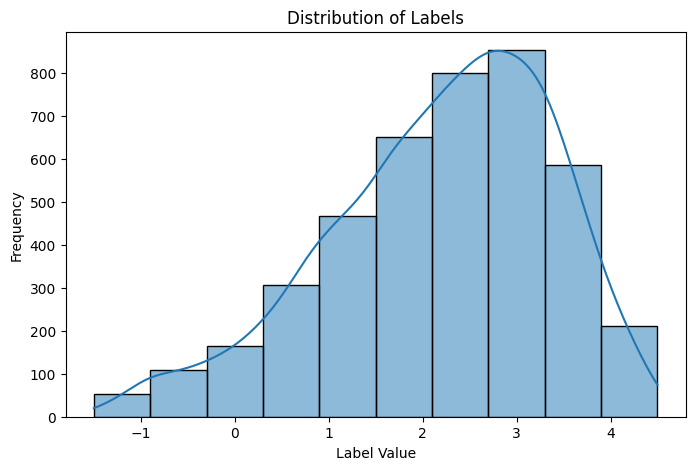
\includegraphics[width=0.4\textwidth]{data-distrib.png} % Adjust width as needed
    \caption{Distribution of the lipophlicity values} % Add a caption if desired
    \label{fig:data-distrib} % Add a label for referencing
\end{figure}

Each model used in this study consists of two components: a language model and a regression head, the latter implemented as a Multi-Layer Perceptron (MLP). The language model employed is MoLFormer \cite{ross2022large}, a pretrained large-scale molecular language model. Each SMILES string is tokenized and processed through MoLFormer, generating an embedding vector, which serves as the input to the regression head responsible for the regression task.

To obtain the best-performing model (the regression head), we employed a Bayesian hyperparameter optimization (HPO) algorithm using the TPE sampler, implemented in the Optuna library \cite{10.1145/3292500.3330701}. The objective of the HPO process was to identify the optimal values for the number of layers, number of neurons per layer, activation function, dropout rates, and learning rate. The algorithm was run for 200 trials, each consisting of 20 epochs, with the goal of minimizing the Mean Squared Error (MSE). The resulting regression head and its performance metrics are presented in Table \ref{tab:regression_head}.

\begin{table}[h]
    \centering
    \caption{Optimal Regression Head Structure from Best Trial}
    \label{tab:regression_head}
    \begin{tabular}{l c}
        \hline
        \textbf{Hyperparameter} & \textbf{Value} \\
        \hline
        Number of Layers ($n_{\text{layers}}$) & 4 \\
        Units in Layer 0 ($n_{\text{units},0}$) & 407 \\
        Activation Function & ELU \\
        Dropout in Layer 0 ($\text{dropout}_0$) & 0.382 \\
        Units in Layer 1 ($n_{\text{units},1}$) & 427 \\
        Dropout in Layer 1 ($\text{dropout}_1$) & 0.278 \\
        Units in Layer 2 ($n_{\text{units},2}$) & 240 \\
        Dropout in Layer 2 ($\text{dropout}_2$) & 0.462 \\
        Units in Layer 3 ($n_{\text{units},3}$) & 69 \\
        Dropout in Layer 3 ($\text{dropout}_3$) & 0.450 \\
        Learning Rate (lr) & 0.0201 \\
        \hline
        \textbf{Best Trial (MSE) Value} & \textbf{0.4050} \\
        \hline
    \end{tabular}
\end{table}

After obtaining the best-performing regression head, we froze the parameters of the language model and utilized its representational knowledge for the downstream task, training only the regression head. This model serves as our baseline for evaluating the effectiveness of the data selection strategies and fine-tuning methods discussed. 

Upon establishing the baseline model, we fine-tuned the language model utilizing masked language modeling (MLM). This approach is designed to enhance the language model's ability to acquire a robust representational understanding of SMILES strings by predicting masked tokens within the sequences. The MLM process was conducted over 4 epochs with a learning rate of 1.6e-4, employing the Adam optimizer. The relatively small learning rate and limited number of epochs were selected to mitigate the risk of overfitting, given the transformer-based language model's propensity to overfit on smaller datasets.

Subsequently, leveraging the fine-tuned language model obtained through MLM, we proceeded to train the regression head. During this phase, the parameters of the language model remained frozen to isolate and evaluate the specific impact of the masked language modeling on the overall performance. This methodological approach ensures a clear assessment of the contribution of MLM to the model's predictive capabilities.

Before conducting the subsequent experiments, we employed three distinct data selection strategies, as detailed in Section \ref{data-selection} on the extra dataset which included 300 data points. The first strategy involves the use of influence functions to identify influential data points. As previously discussed, constructing and inverting the Hessian matrix is computationally expensive. To address this, we utilized the LiSSA (Linear (time) Stochastic Second-Order Algorithm) method to approximate the inverse Hessian-vector product. For the LiSSA algorithm, we set the recursive depth to 2 and used 2 independent samples to balance computational efficiency and approximation accuracy. To compute the influence scores, we utilized the trained regression head in conjunction with the language model fine-tuned through masked language modeling (MLM). 

Influential data points can significantly impact the model's predictive performance. Therefore, we selected data points whose influence scores were either greater than the mean plus half the standard deviation or less than the mean minus half the standard deviation as depicted in figure \ref{fig:influence-distrib}. This criterion ensures that only data points with a substantial effect on the loss value are retained, thereby enhancing the model's robustness and performance. After filtering out the non-influential data points, a total of 36 data points remained, constituting 12\% of the total number of additional data points.

\begin{figure}[htbp]
    \centering
    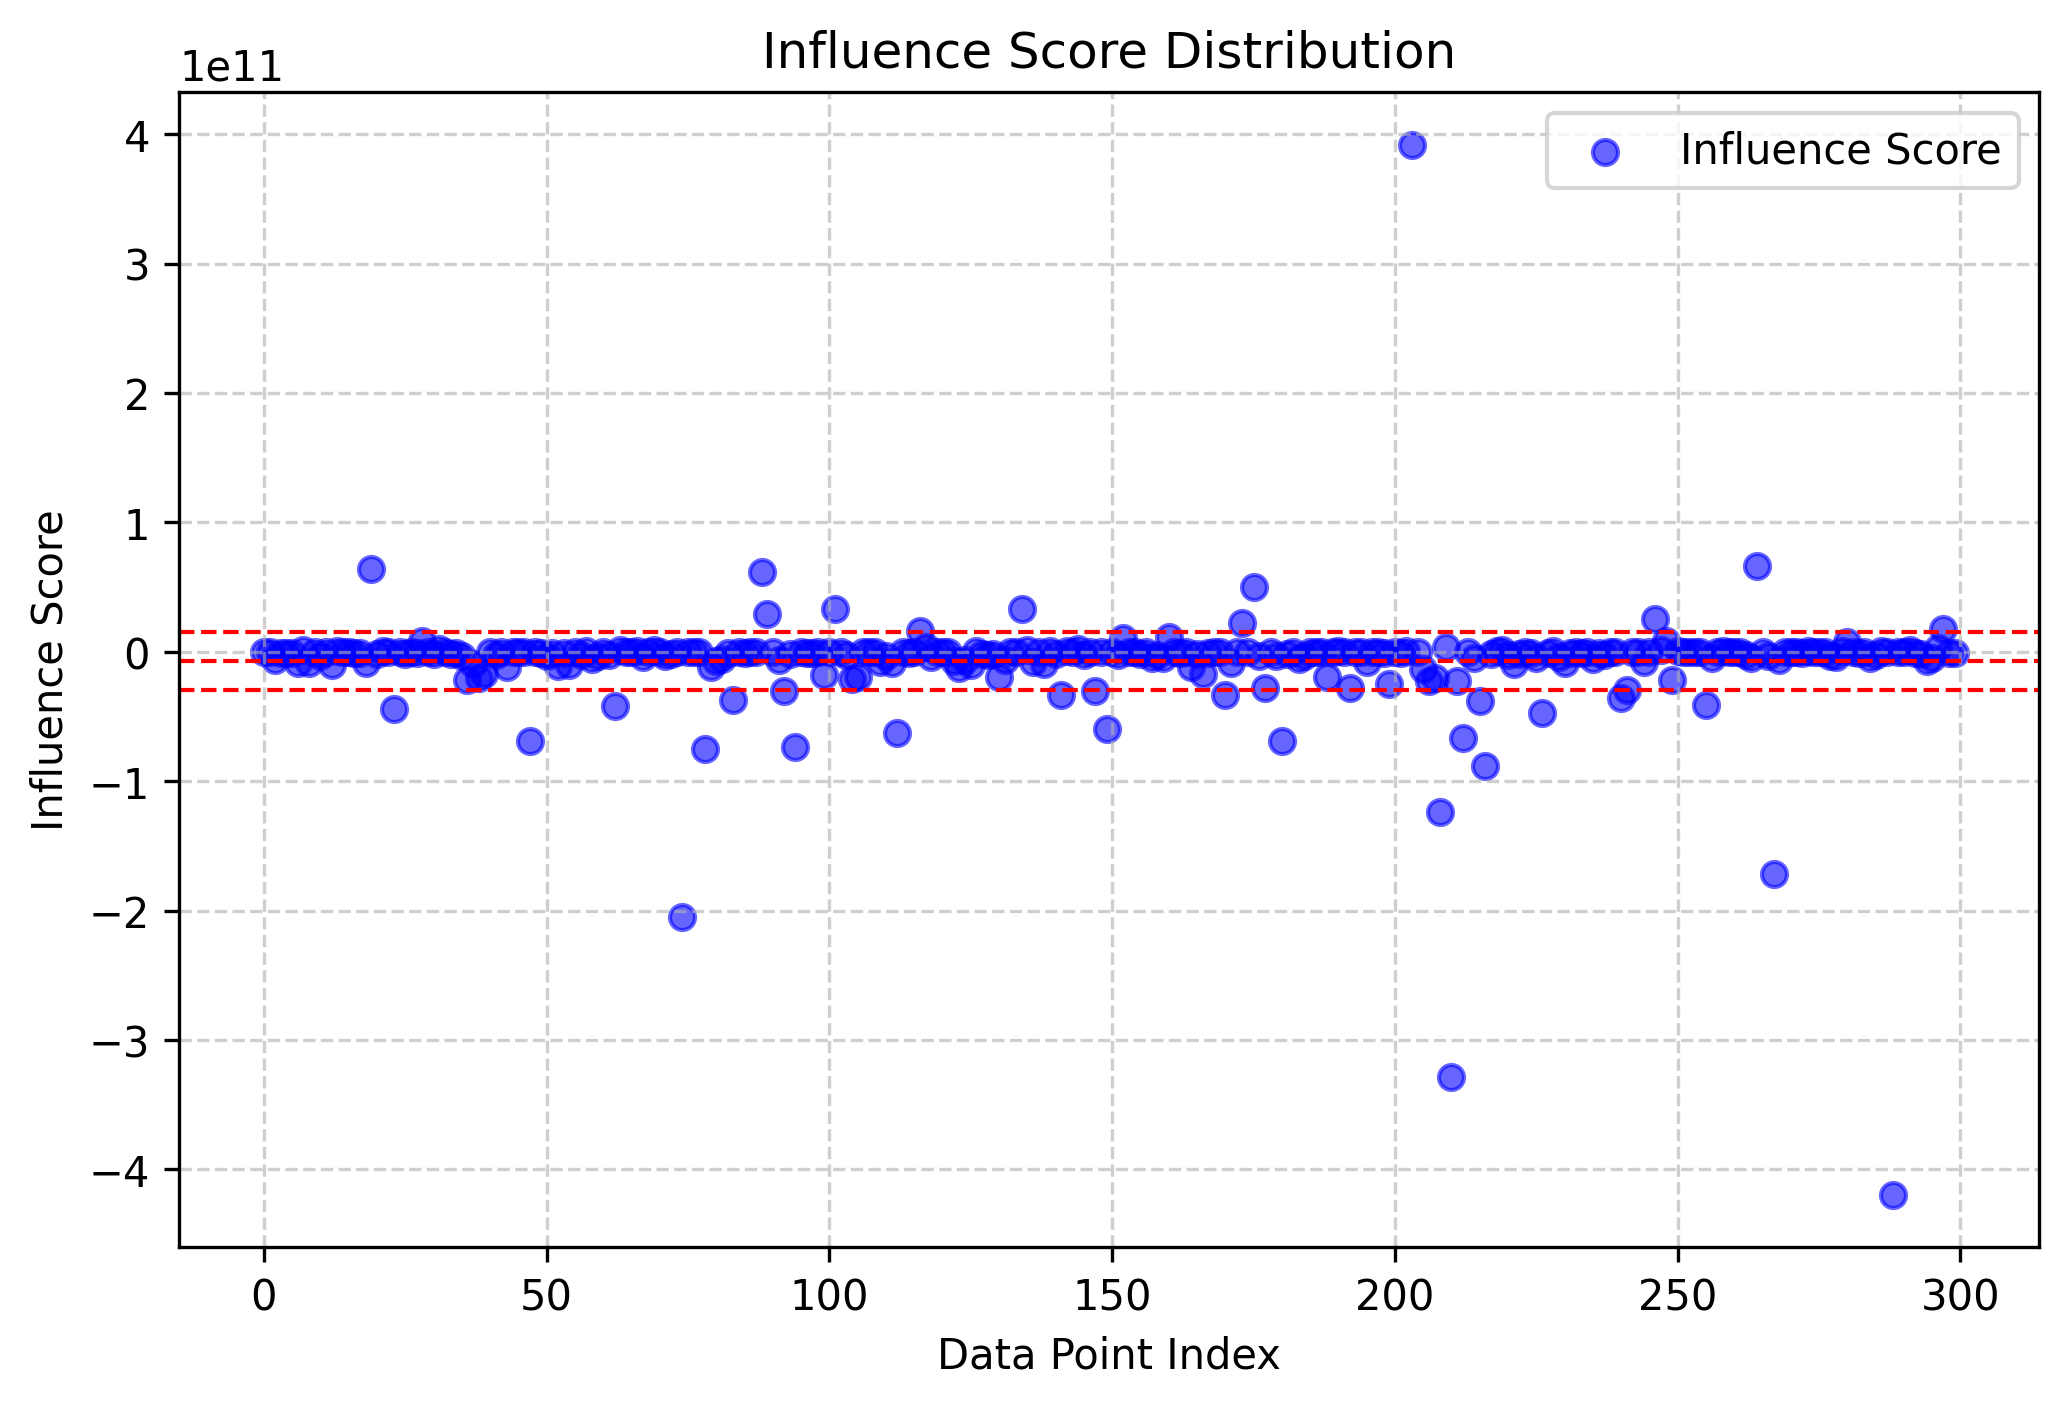
\includegraphics[width=0.4\textwidth]{influence_scatter_plot.png} 
    \caption{Distribution of influence scores across all data points. The central line indicates the mean influence score, while the upper and lower lines represent thresholds set at half the standard deviation above and below the mean, respectively.} % Add a caption if desired
    \label{fig:influence-distrib} 
\end{figure}

To evaluate the impact of uncertainty-based data selection, we applied variance-based selection to the external lipophilicity dataset which consisted of 300 additional points. The uncertainty of each sample was estimated by computing the variance of model predictions across multiple inferences. The top 10\% most uncertain samples were selected and incorporated into the training dataset. This approach led to a reduction in Mean Squared Error (MSE) compared to training with the full dataset, demonstrating that prioritizing uncertain samples enhances generalization. The model benefited from focusing on challenging samples, leading to improved robustness in lipophilicity prediction. In other words, this method ensures that the model learns from its own weaknesses. These findings align with prior research, suggesting that uncertainty-aware selection strategies improve model performance by reducing overfitting and guiding learning towards underrepresented molecular structures\cite{nigam2021assigning}.

We also employed the Small-to-Large (S2L) strategy, which selects informative samples based on their loss trajectories. A small proxy model, \texttt{EleutherAI/pythia-70m}, was trained on the dataset, and loss trajectories were recorded for each sample, following the methodology outlined in \cite{yang2023small}. To identify samples with similar learning difficulty, we applied K-Means clustering to group the data into three distinct clusters. From each cluster, a balanced subset of samples was selected, ensuring that 10\% of the external data was incorporated while maintaining diversity in the final dataset.  




We trained the regression head using the language model fine-tuned with masked language modeling (MLM), while keeping its weights frozen. This training was performed on a combined dataset consisting of the main dataset and the selected data points from each of the three data selection strategies. We evaluated the performance of each combination and selected the one that yielded the best results for use in subsequent fine-tuning experiments. Specifically, we trained three distinct models, each corresponding to a different data selection strategy, and chose the data combination that demonstrated the highest performance for the fine-tuning tasks.

In this experiment, we employed three fine-tuning methods: BitFit \ref{BitFit}, LoRA \ref{LoRA}, and (IA)$^3$ \ref{iA3}. Using the best-performing data combination identified in the previous experiment, we fine-tuned the language model with each of these methods. The fine-tuning approach that achieved the highest performance was selected for use in our final experiment.

In the final experiment, we explored the impact of incorporating additional molecular knowledge by introducing a second input to the model. This input enables the model to learn a shared representation of both SMILES strings and molecular features. We utilized a 7-dimensional vector as the second input, which includes the following molecular descriptors: molecular weight, number of hydrogen bond donors, number of hydrogen bond acceptors, topological polar surface area (TPSA), molar refractivity, formal charge, and fraction of sp$^3$-hybridized carbon atoms. These features were selected due to their conceptual relevance to lipophilicity, as their inclusion could potentially enhance the model's performance by enriching its understanding of molecular properties.

In this experiment, the output of the language model was fed into the regression head described in Table \ref{tab:regression_head}. Additionally, the 7-dimensional molecular feature vector was processed through a multilayer perceptron (MLP) network. The outputs of both the regression head and the MLP were concatenated and subsequently passed through a fully connected layer to perform the final regression task.

All experiments were conducted using the Adam optimizer and the mean squared error (MSE) loss function, with training performed for 40 epochs unless otherwise specified. The models were trained on an Nvidia GeForce GTX 1650 Ti GPU, utilizing the PyTorch framework \cite{NEURIPS2019_bdbca288} (version 2.2.0) for implementing the machine learning models.

\subsection{Analysis and Findings}
\label{analysis}
The experimental results discussed in Section \ref{experiments} are presented in Table \ref{tab:rmse_loss}. We initially conducted experiments using the raw language model without any fine-tuning and trained the regression head on the MoleculeNet dataset while keeping the language model weights frozen. The baseline performance achieved a root mean squared error (RMSE) loss of 0.813 on the training set and 0.780 on the test set. Applying masked language modeling to the language model did not improve the baseline performance and instead yielded slightly worse results. The most likely explanation for this outcome is that MolFormer is already pre-trained on millions of SMILES strings from the PubChem and ZINC datasets. Consequently, further training on an additional 4,200 data points using masked language modeling is unlikely to produce significant improvements. However, as evident in Figure \ref{fig:Raw-vs-MLM}, training the model after masked language model fine-tuning results in significantly smoother train-test loss curves compared to training on the raw model.

\begin{figure}[htbp]
    \centering
    \begin{minipage}{0.48\textwidth}
        \centering
        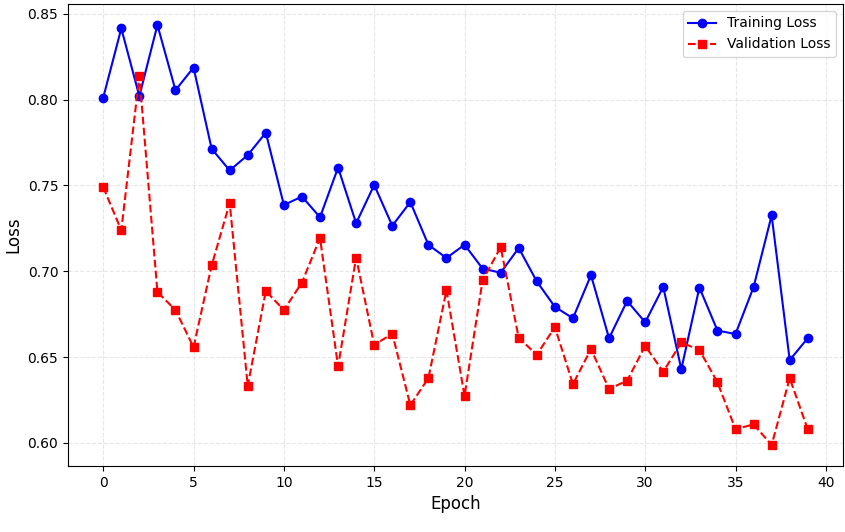
\includegraphics[width=\textwidth]{LM_RAW.png} % Adjust width as needed
    \end{minipage}
    \hfill
    \begin{minipage}{0.48\textwidth}
        \centering
        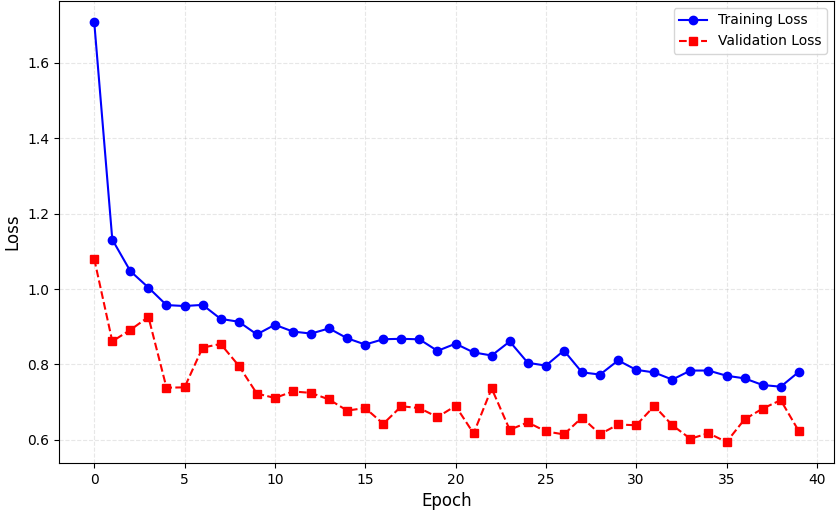
\includegraphics[width=\textwidth]{LM_MLM.png}  
    \end{minipage}
    \caption{Training and validation loss for (up) the raw language model versus (down) the language model fine-tuned using MLM. The values represent Mean Squared Error (MSE).} 
    \label{fig:Raw-vs-MLM} 
\end{figure}

In the next step, we employed an MLM pre-trained language model to evaluate various data selection strategies. The data selection process was conducted on an additional set of 300 data points, which were then combined with our primary dataset of 4,200 data points to train the model. For the language model, we utilized the MLM pre-trained version, keeping its weights frozen and only training the regression head. We tested three data selection strategies across four experiments, with the uncertainty-based selection strategy achieving the best results, yielding an RMSE of 0.859 on the training set and 0.809 on the test set. The uncertainty method required only a single forward pass, making it computationally more efficient compared to the influence function approach while also delivering superior performance. The train and validation loss curve is depicted in Figure \ref{fig:uncertainty}.  


In the next step, we employed an MLM pre-trained language model to evaluate various data selection strategies. The data selection process was conducted on an additional set of 300 data points, which were then combined with our primary dataset of 4,200 data points to train the model. For the language model, we utilized the MLM pre-trained version, keeping its weights frozen and only training the regression head. We tested three data selection strategies across four experiments, with the uncertainty-based selection strategy achieving the best results, yielding an RMSE of 0.859 on the training set and 0.809 on the test set.


The uncertainty method required only a single forward pass, making it computationally more efficient compared to the influence function approach while also delivering superior performance. Compared to the Small-to-Large (S2L) method, which selects a balanced mix of easy, medium, and hard samples based on loss trajectories, the uncertainty-based approach focused directly on the most informative and underrepresented data points, those with the highest variance in predictions. This targeted selection strategy proved particularly effective for molecular property prediction, as it helped reduce dataset biases and improve generalization. In contrast, the loss-based clustering in S2L did not always align with molecular complexity in a regression task, potentially leading to the inclusion of redundant or less informative samples. Additionally, since the proxy model used for loss computation in S2L was relatively small, it may not have captured the same feature representations as the full-scale MoLFormer, limiting its effectiveness. While S2L remains a promising data selection strategy, its performance in this task suggests that uncertainty-based methods may be better suited for improving transformer-based molecular property prediction. The train and validation loss curve is depicted in Figure \ref{fig:uncertainty}.



\begin{figure}[htbp]
    \centering
    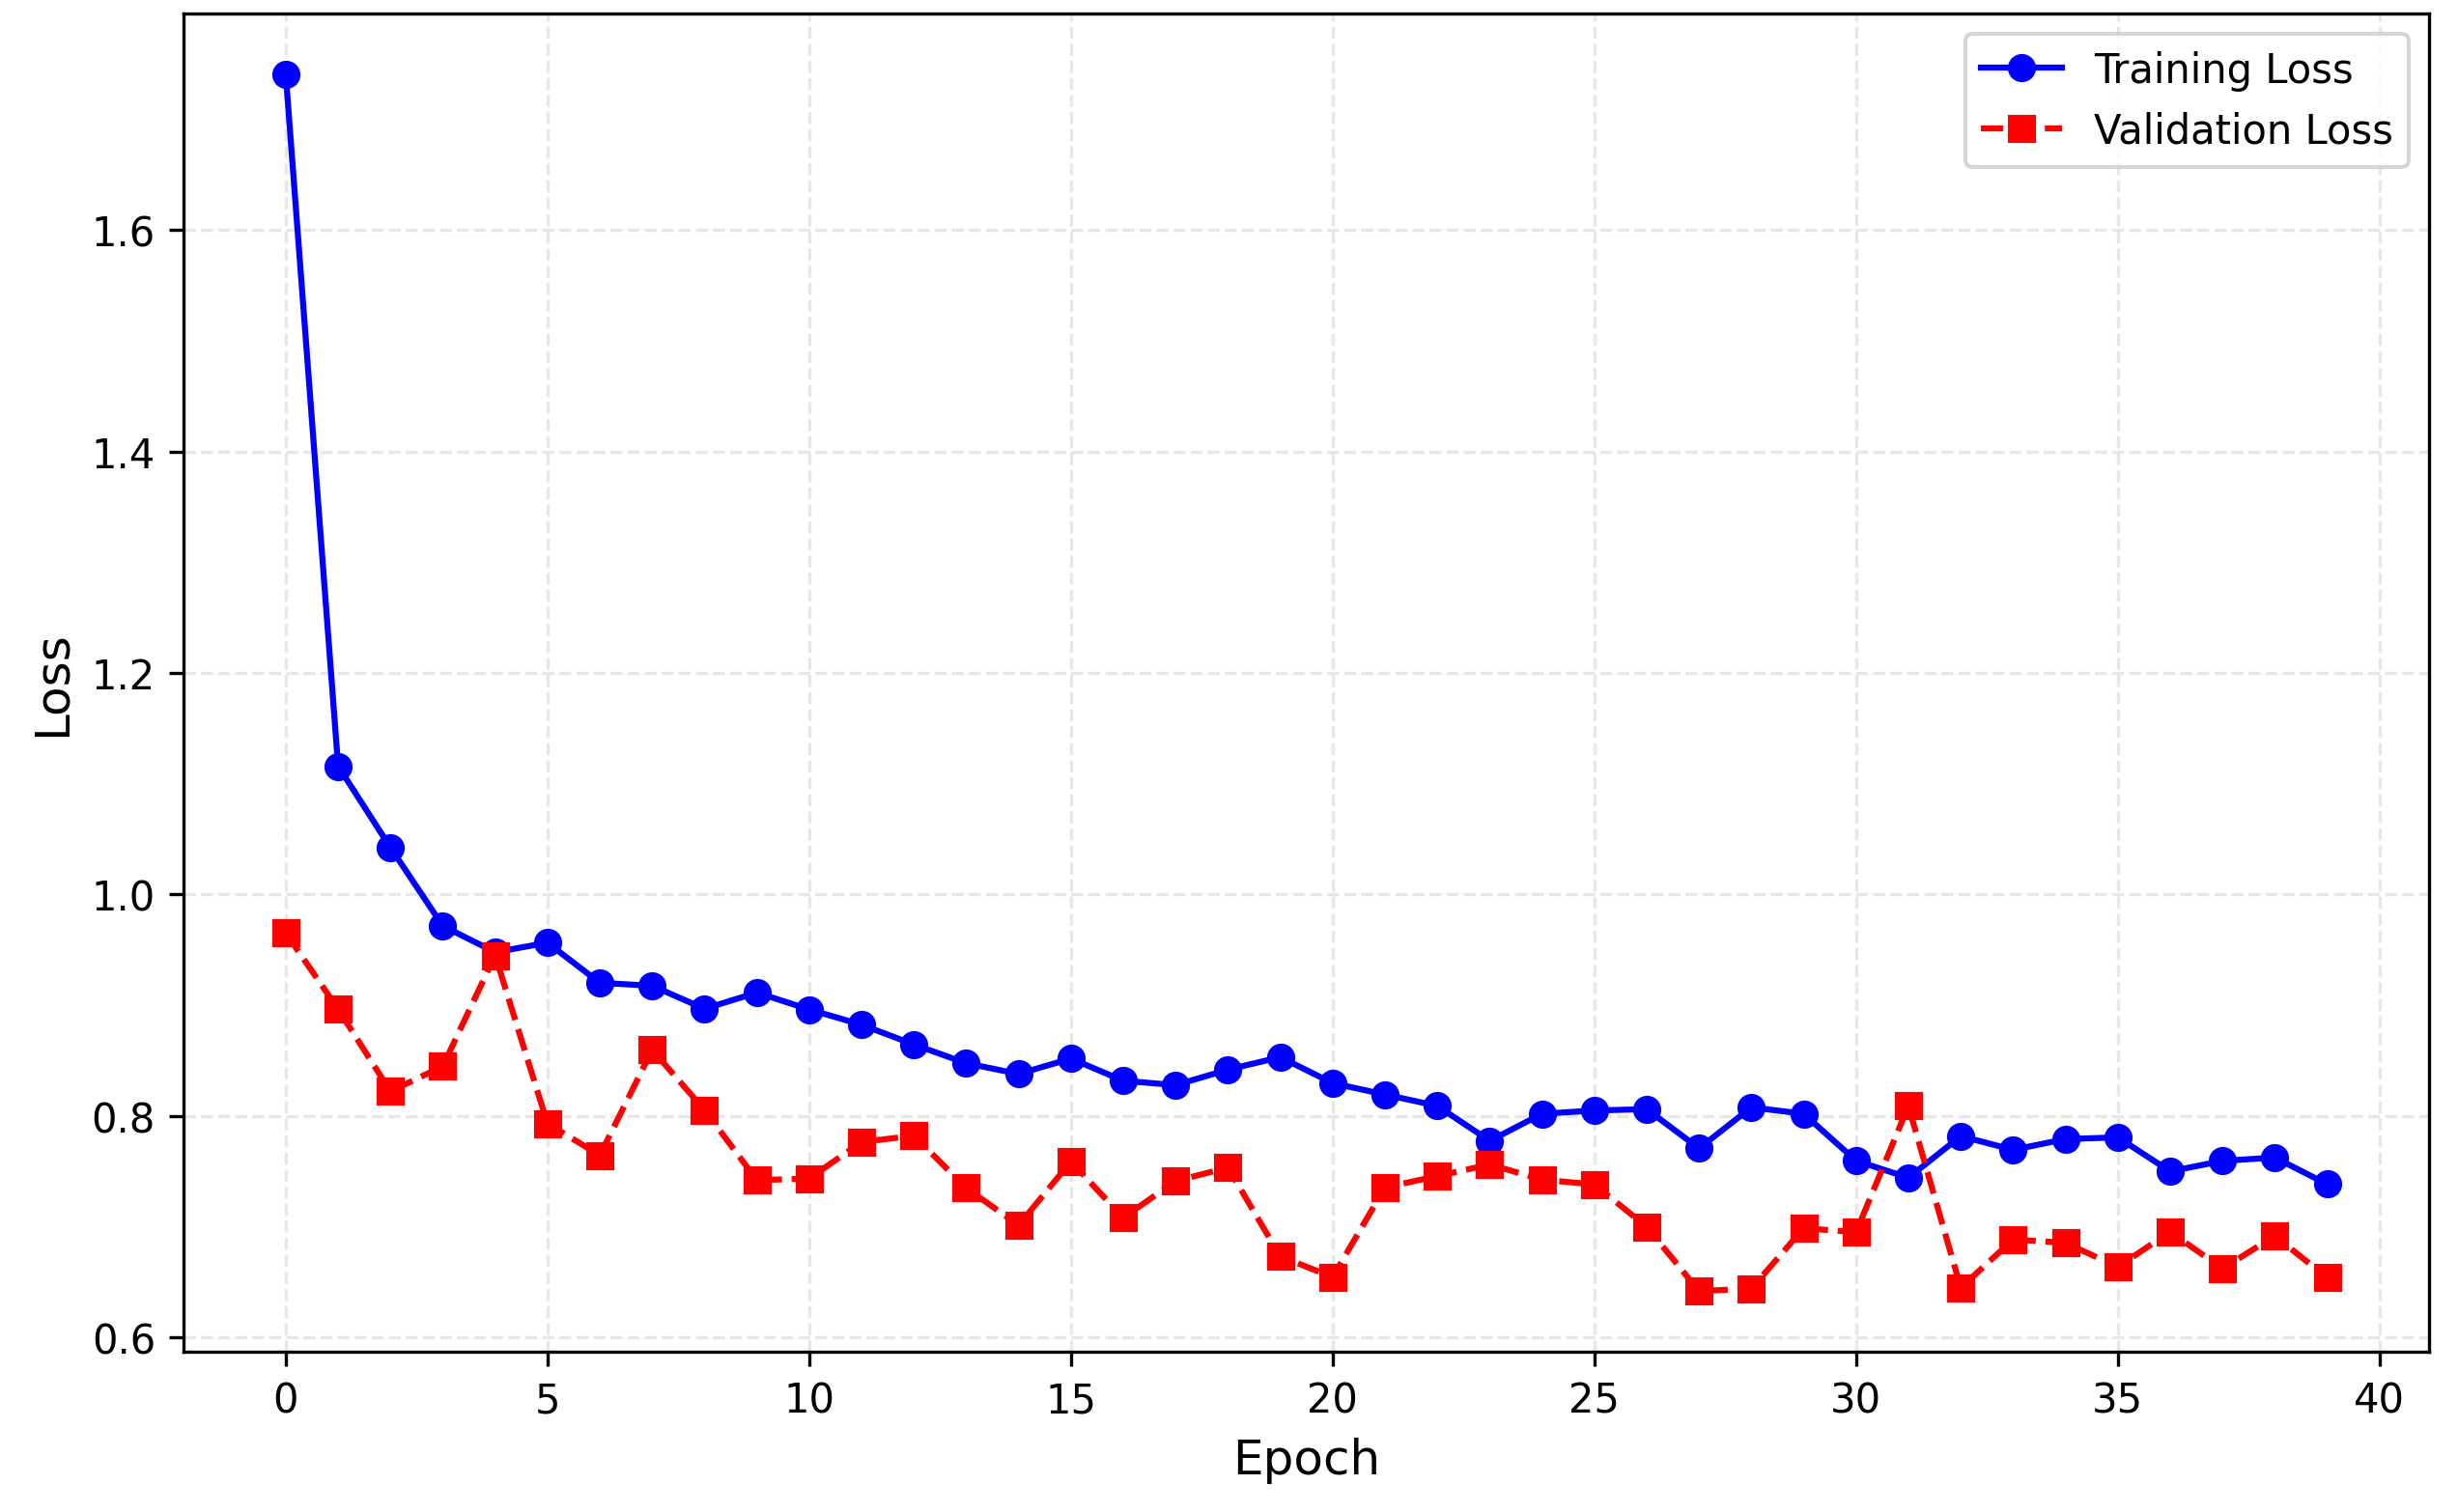
\includegraphics[width=0.5\textwidth]{LM_Uncertainty.png} 
    \caption{Train and Validation MSE Loss curve for training MLM fine-tuned model using uncertainty selected data.} % Add a caption if desired
    \label{fig:uncertainty} 
\end{figure}

To evaluate various fine-tuning methods, we combined the uncertainty-selected data points with our main dataset. Among the three fine-tuning methods tested, BitFit achieved the best results, with an RMSE loss of 0.722 on the training set and 0.690 on the test set, representing a significant improvement over the baseline. Given the limited size of our downstream task dataset, BitFit proved to be the most effective solution, as it only updates the bias parameters without requiring additional parameters to be added. A key advantage of BitFit is its efficiency, as it modifies only the bias terms, making it both lightweight and computationally efficient. The combination of the uncertainty-selected dataset and the model fine-tuned using BitFit represents the best-performing configuration, as highlighted in Table \ref{tab:rmse_loss}. Moreover, the loss curve for this combination can be seen in Figure \ref{fig:BitFit-Uncertainty}.

\begin{figure}[htbp]
    \centering
    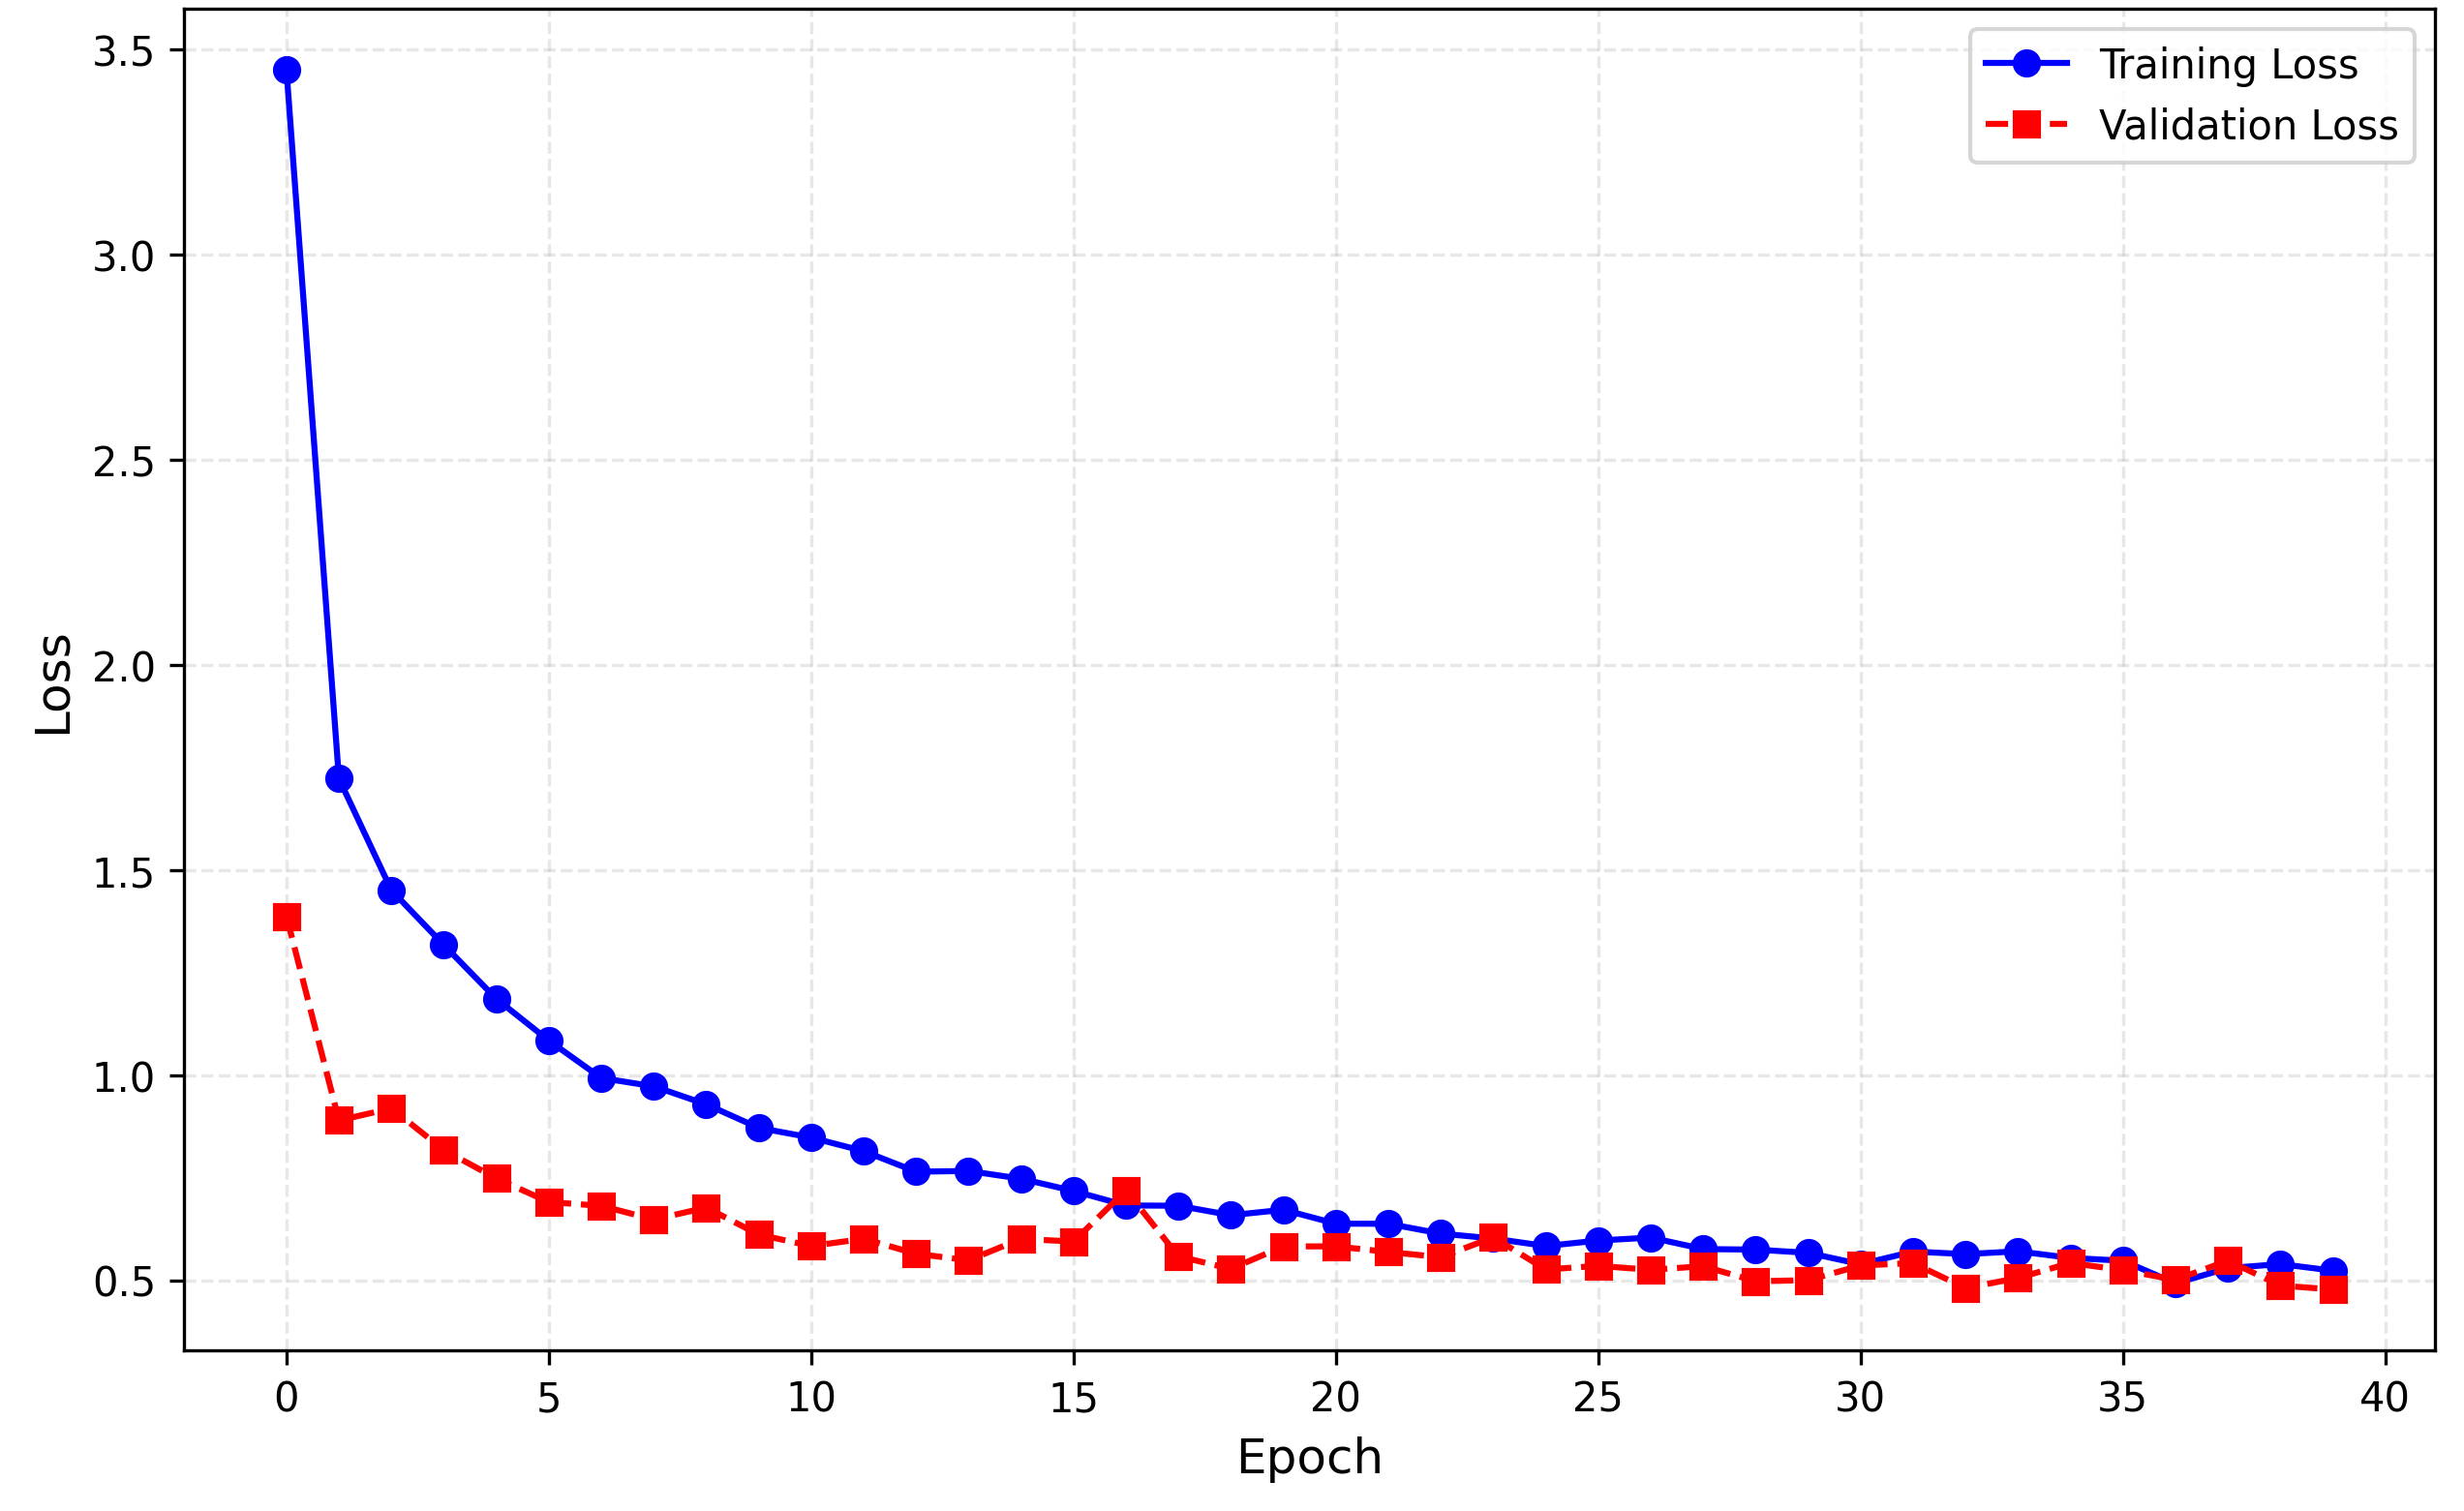
\includegraphics[width=0.5\textwidth]{BitFit_Uncertainty.png} 
    \caption{Train and Validation MSE loss for model fine-tuned with BitFit using uncertainty selected data.} % Add a caption if desired
    \label{fig:BitFit-Uncertainty} 
\end{figure}

To assess the impact of incorporating additional domain knowledge and to evaluate the shared representation of SMILES embeddings combined with a 7-dimensional feature vector, we implemented a multi-input model. Train and validation loss can be seen in figure \ref{fig:Multi-Input}. While this approach did not outperform the BitFit fine-tuned model (achieving an RMSE of 0.728 on the training set and 0.756 on the test set), further investigation is warranted. Specifically, conducting hyperparameter optimization, as done earlier in this study, could potentially lead to significant improvements in baseline performance.

\begin{figure}[htbp]
    \centering
    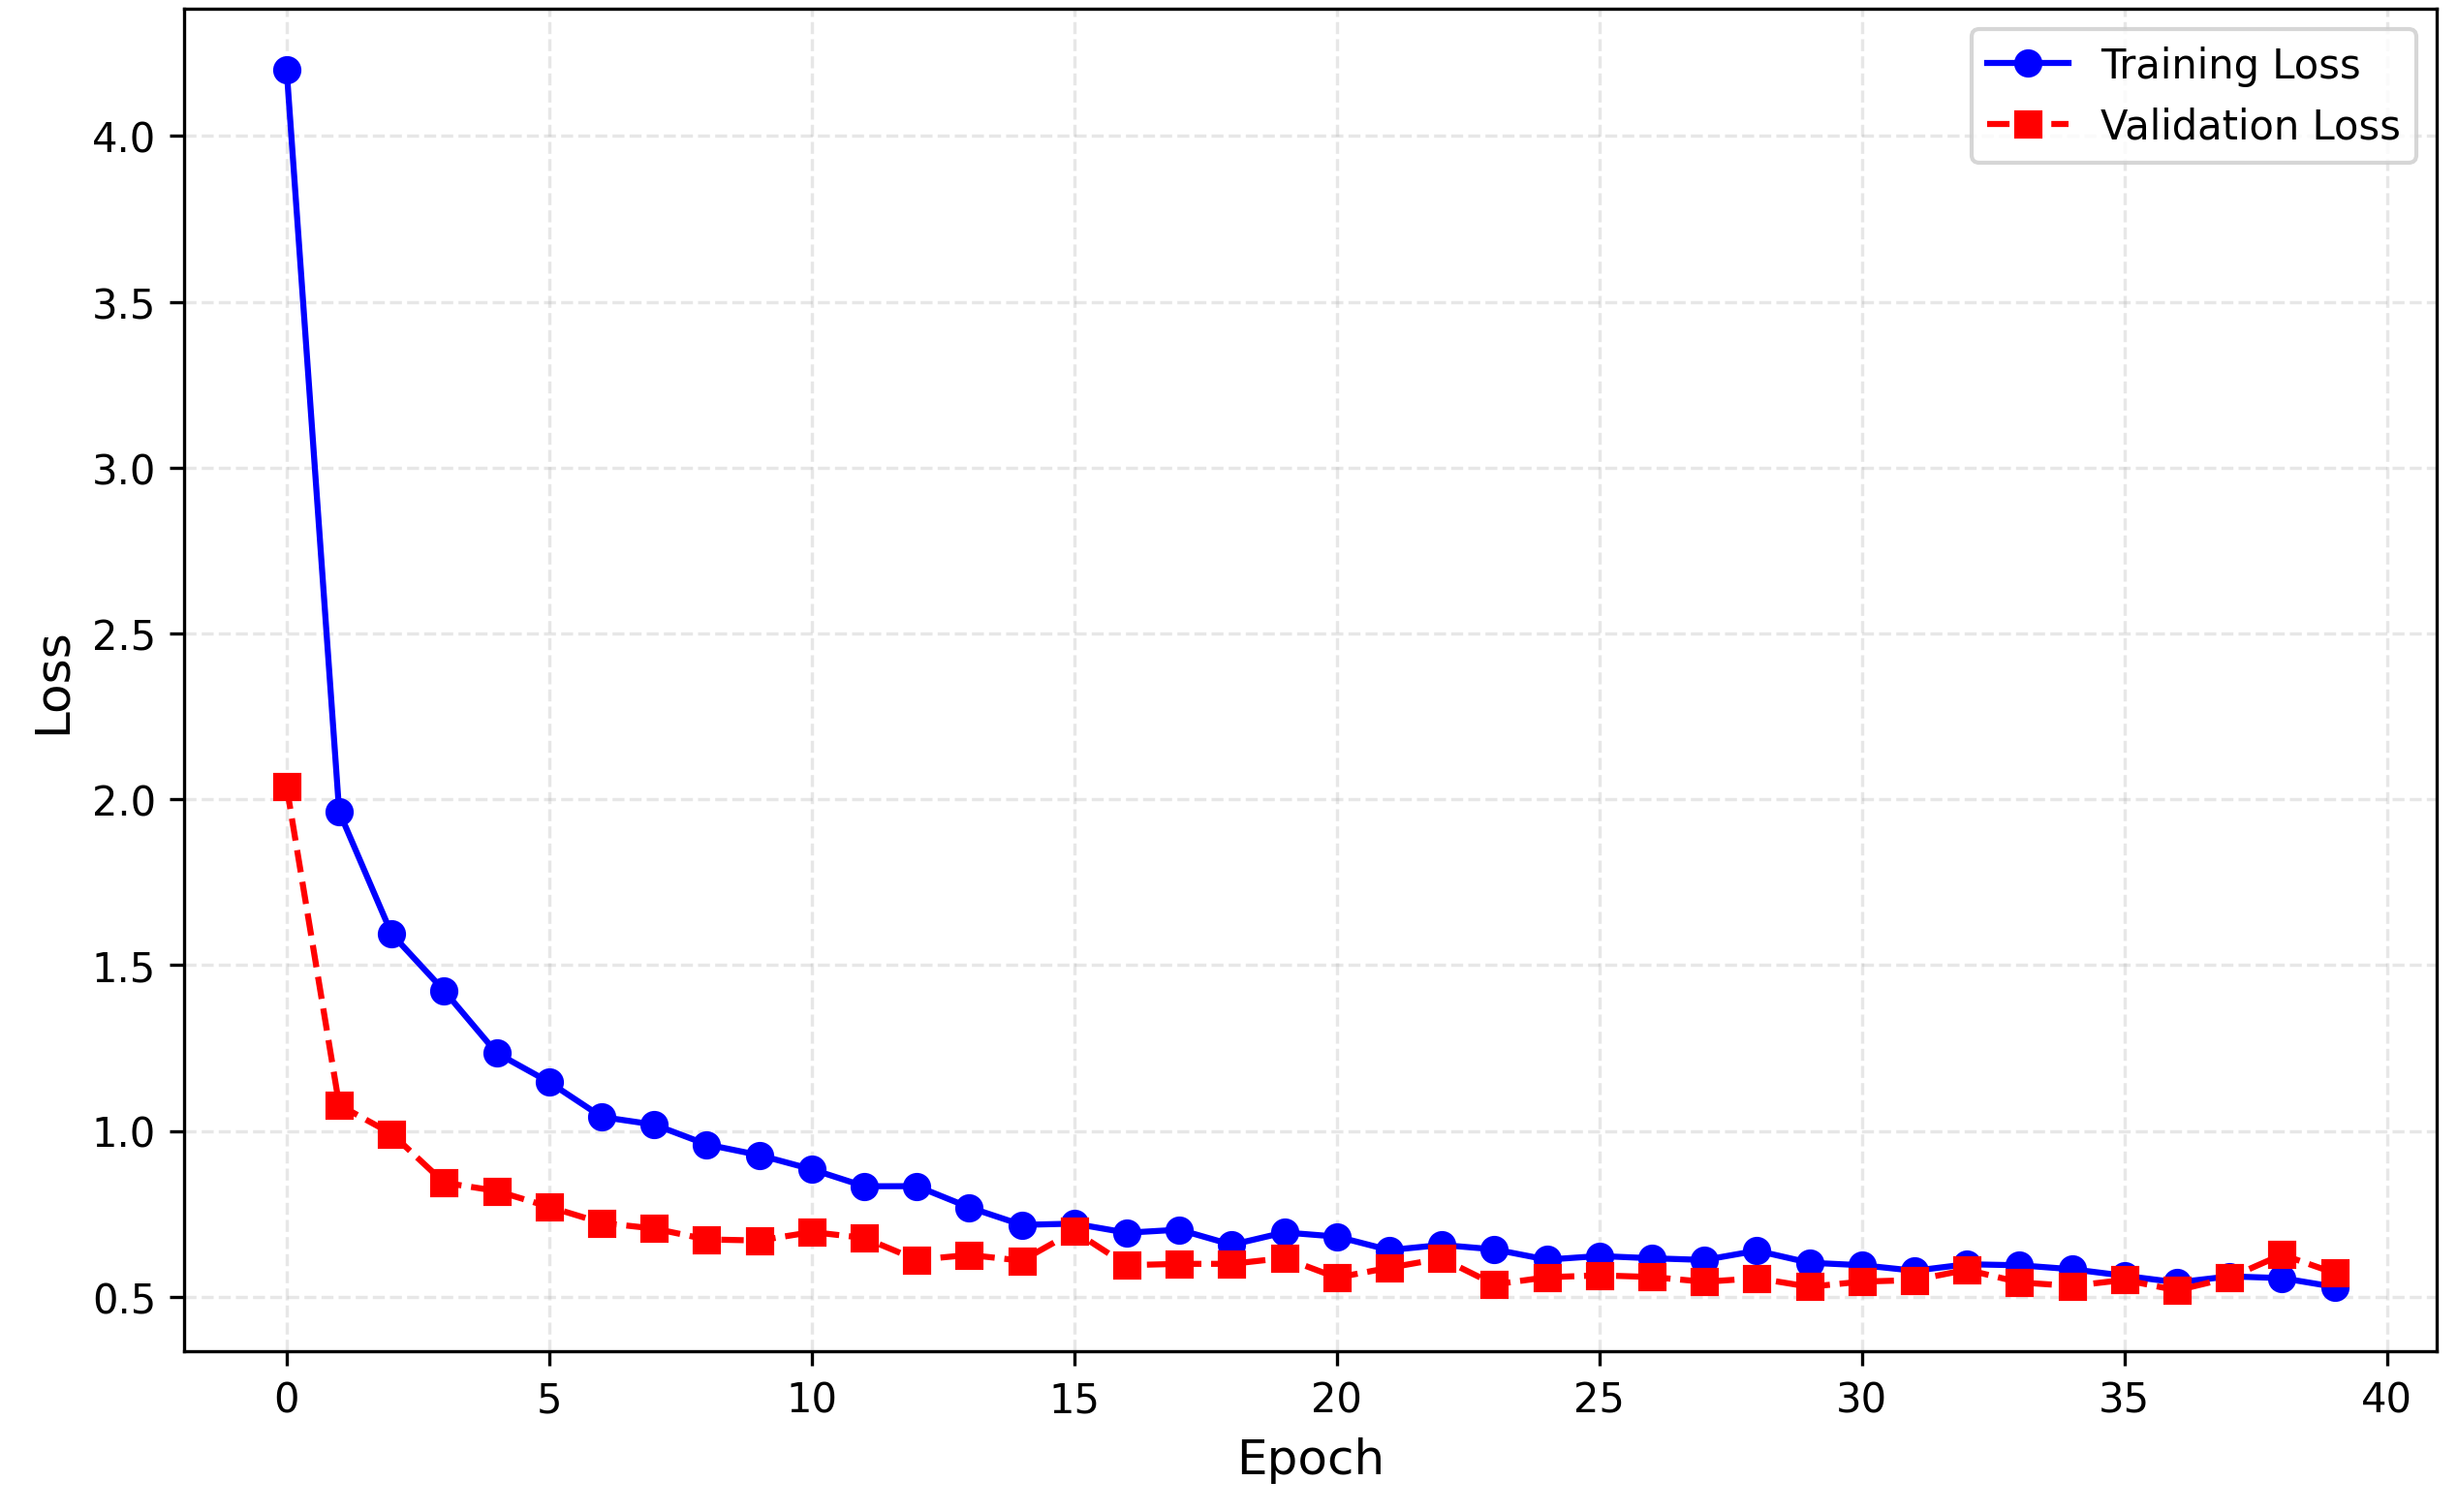
\includegraphics[width=0.5\textwidth]{Multi-Input.png} 
    \caption{Train and Validation MSE loss for multi-input model.}
    \label{fig:Multi-Input} 
\end{figure}

\begin{table*}[t]
\centering
\begin{tabular}{lrr}
\toprule
\textbf{Model} & \textbf{Train Loss} & \textbf{Validation Loss} \\
\midrule
LM (Raw) + Regression Head & 0.813 & 0.780 \\
\midrule
LM (MLM) + Regression Head & 0.883 & 0.789 \\
LM (MLM) + Regression Head (Uncertainty) & 0.859 & 0.809 \\
LM (MLM) + Regression Head (S2L-30) & 1.233 & 1.203 \\
LM (MLM) + Regression Head (S2L-100) & 0.838 & 0.866 \\
LM (MLM) + Regression Head (Influence) & 0.868 & 0.838 \\
\midrule
LM (BitFit) + Regression Head (Uncertainty) & \textbf{0.722} & \textbf{0.690} \\
LM (LoRA) + Regression Head (Uncertainty) & 0.911 & 0.884 \\
LM (iA3) + Regression Head (Uncertainty) & 0.761 & 0.765 \\
\midrule
LM (BitFit) + Multi-input Model (Uncertainty) & 0.728 & 0.756 \\
\bottomrule
\end{tabular}
\caption{Root Mean Squared Error (RMSE) Loss for various model configurations. Parentheses after ``LM'' indicate the fine-tuning method applied to the language model. The model structure, either a simple regression head or a multi-input model, is specified after the plus sign. Parentheses at the end of each model name denote the data selection strategy used during testing.}
\label{tab:rmse_loss}
\end{table*}

\section{Conclusions and Future Directions}

In this study, we explored the impact of data selection and fine-tuning methods on the task of predicting lipophilicity data. Using SMILES strings as input to our language model, we constructed a regression head on top of the model to predict lipophilicity values. The lipophilicity dataset from the MoleculeNet benchmark served as our primary dataset, with MolFormer employed as the language model. Additionally, we utilized an extra 300 data points to evaluate the effectiveness of various data selection strategies, including Influence Functions, S2L, and the uncertainty method. Our results demonstrated that the uncertainty-based data selection strategy outperformed the other methods.

We further investigated several fine-tuning approaches, such as Masked Language Modeling (MLM), BitFit, LoRA, and (IA)$^3$. Among these, BitFit significantly improved baseline performance, surpassing the other methods. 

As a final experiment, we developed a multi-input model to explore the integration of domain knowledge. A 7-dimensional feature vector was created using the RDKit library to augment the model's input. 

For future work, we recommend further investigation into the use of domain knowledge and the development of a more effective multi-input model. Techniques such as Bayesian Optimization, as employed in this study, could be leveraged for hyperparameter tuning to enhance performance. Furthermore, exploring Monte Carlo (MC) Dropout as an alternative uncertainty-based data selection method could be useful. Unlike single-pass variance estimation, MC Dropout enables epistemic uncertainty estimation by performing multiple stochastic forward passes through the model with dropout activated. This approach captures uncertainty by generating diverse predictions for the same input and computing their variance, helping to identify uncertain samples. It would be beneficial to explore the effectiveness of this method in sample selection in chemical space.



% Entries for the entire Anthology, followed by custom entries
\bibliography{anthology,custom}
\bibliographystyle{acl_natbib}


\end{document}
